\chapter{Timing, in full}
\label{ch:timing}

Chapters~\ref{sec:avg}--\ref{sec:stream} gave each method's budget. This chapter
gives the evidence that the model behind them is right, and the practical
consequences.

\section{The evidence for a per-call floor}
\label{sec:floorevidence}

Applying the exact-recovery technique of \S\ref{sec:quantum} to all 21 usable
averaged runs across three sessions (\file{tables/timing.csv}):

\begin{center}
\small
\begin{tabular}{@{}llrrrr@{}}
\toprule
\hd{Session} & \hd{Config} & \hd{ADC integration} & \hd{Fastest call} & \hd{Median period} & \hd{Rate} \\
\midrule
2026-08-04 & $D$=654340  & \SI{4.26}{\milli\second} & 9.35--\SI{9.53}{\milli\second} & 10.48--\SI{10.62}{\milli\second} & 94--95\,Hz \\
2026-08-04 & $D$=706560  & \SI{4.60}{\milli\second} & \SI{9.29}{\milli\second} & \SI{10.84}{\milli\second} & 92\,Hz \\
2026-08-04/06 & $D$=1504982 & \SI{9.80}{\milli\second} & 9.61--\SI{10.29}{\milli\second} & 10.93--\SI{11.54}{\milli\second} & 87--91\,Hz \\
\textbf{2026-08-14} & $D$=368640 & \textbf{\SI{2.40}{\milli\second}} & 10.14--\SI{10.30}{\milli\second} & 11.26--\SI{11.52}{\milli\second} & 87--89\,Hz \\
\textbf{2026-08-14} & $D$=847872 & \textbf{\SI{5.52}{\milli\second}} & \SI{10.27}{\milli\second} & \SI{11.39}{\milli\second} & 87.8\,Hz \\
\bottomrule
\end{tabular}
\end{center}

Two runs were excluded from the fit below because their loop period exceeds
1.5$\times$ their acquire time --- most of it was spent outside \co{acquire()}
(live plotting on, or operator interaction), so they say nothing about the call.

\begin{figure}[H]
\centering
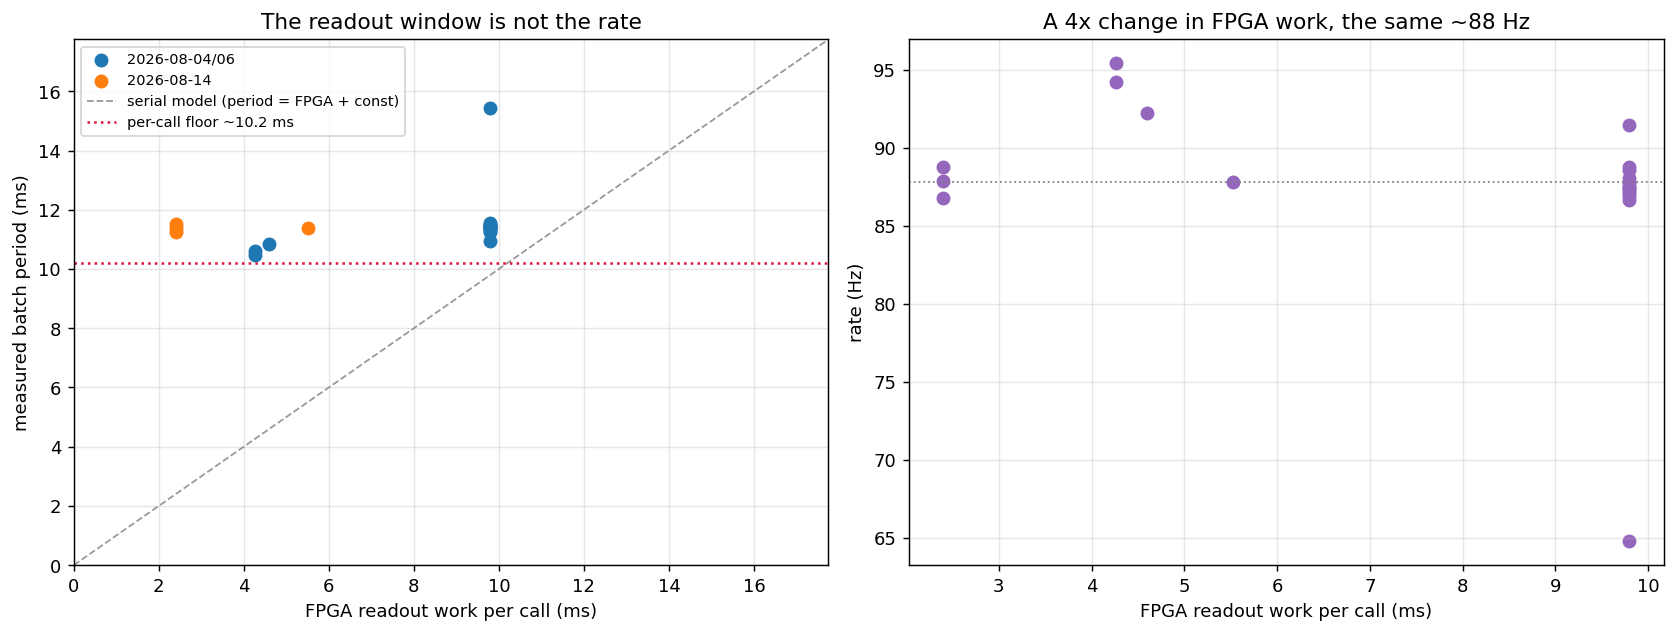
\includegraphics[width=\linewidth]{figures/timing_floor.png}
\caption{Left: measured batch period against FPGA readout work. The dashed line is
the serial model the data does not follow; the red dotted line is the per-call
floor. Right: the same data as rate --- a 4$\times$ change in FPGA work leaves the
rate at $\sim$88\,Hz.}
\end{figure}

\subsection{Argument 1 --- the slope is not 1}

Fitted \emph{within} a session, because comparing across sessions would confound
the FPGA change with the floor itself, which moved $\sim$1\,ms between 2026-08-04/06
and 2026-08-14:

\begin{center}
\small
\begin{tabular}{@{}lrrr@{}}
\toprule
\hd{Session} & \hd{FPGA work} & \hd{Period} & \hd{$d(\text{period})/d(\text{FPGA})$} \\
\midrule
2026-08-04/06 & 4.26 $\rightarrow$ \SI{9.80}{\milli\second} (2.3$\times$) & 10.55 $\rightarrow$ \SI{11.43}{\milli\second} & \textbf{+0.140} \\
2026-08-14    & 2.40 $\rightarrow$ \SI{5.52}{\milli\second} (2.3$\times$) & 11.38 $\rightarrow$ \SI{11.39}{\milli\second} & \textbf{+0.003} \\
\bottomrule
\end{tabular}
\end{center}

A serial model $\text{period} = \text{host} + \text{FPGA}$ requires slope
$= 1.000$. Neither session comes close.

\subsection{Argument 2 --- no serial model fits at all}

The 2026-08-14 runs used \SI{2.40}{\milli\second} of FPGA work, and their
\emph{fastest} call was \SI{10.14}{\milli\second}. Under a serial model that
demands a host term of \SI{7.74}{\milli\second}, against the
\SI{1.60}{\milli\second} the 2026-08-06 analysis reported for the same code on the
same rig eight days earlier. There is no constant, non-negative host term that
fits both sessions.

Under the max-model both are consistent: the host chain is $\sim$10--11.4\,ms in
both, and the FPGA work is simply hidden inside it.

\subsection{Argument 3 --- the wobble is entirely in the call}

The instantaneous rate spans 81.4--100.1\,Hz, which is what is seen live as
``85--97\,Hz''. Decomposing it:

\begin{itemize}
  \item The FPGA term is \textbf{deterministic} --- 23 reps of identical pulse work
        vary by well under a microsecond, and the burst runs confirm the cadence is
        stable to 0.4\% across runs.
  \item \co{acq_seconds} spans 10.1--\SI{12.1}{\milli\second} (jitter
        1.6--\SI{1.9}{\milli\second} p95$-$p05).
  \item Python outside the call stays at \SI{0.06}{\milli\second}.
\end{itemize}
So \textbf{100\% of the wobble is host/network scheduling inside \co{acquire()}} ---
Windows scheduling plus TCP/Pyro latency on stages 1--6.

\section{The corrected model}
\label{sec:model}

\begin{equation}
\boxed{\;
\text{period} \;=\; \max\bigl(\underbrace{H}_{\text{host call}},\;
\underbrace{\text{reps}\times t_\text{rep}}_{\text{FPGA}}\bigr) \;+\; \underbrace{P}_{\text{Python, }\sim\SI{0.06}{\milli\second}}
\;}
\label{eq:model}
\end{equation}

with, on this rig,
\[
H_\text{typical} = \SI{11.4}{\milli\second}, \qquad
H_\text{floor} = \SI{10.1}{\milli\second}.
\]

Two constants rather than one, because the two uses want different ends of the
distribution: $H_\text{typical}$ predicts the rate, $H_\text{floor}$ sizes the free
averaging (fill past the fastest call and even the quick calls become FPGA-bound).

\subsection{Predicted against measured}

\begin{center}
\small
\begin{tabular}{@{}llrrrr@{}}
\toprule
\hd{$\tau$} & \hd{reps} & \hd{FPGA} & \hd{Old model} & \hd{Eq.~\ref{eq:model}} & \hd{Measured} \\
\midrule
\SI{213}{\micro\second} & 23 & \SI{9.80}{\milli\second} & 160\,Hz & \textbf{87.7\,Hz} & 87.5\,Hz \\
\SI{120}{\micro\second} & 23 & \SI{5.52}{\milli\second} & 400\,Hz & \textbf{87.7\,Hz} & 87.8\,Hz \\
\SI{120}{\micro\second} & 10 & \SI{2.40}{\milli\second} & 180\,Hz & \textbf{87.7\,Hz} & 86.8\,Hz \\
\bottomrule
\end{tabular}
\end{center}

The model giving the \emph{same} answer for all three is the point.

\co{measure_host_floor()} calibrates $H$ on the rig in about a second, using a
\co{reps=1} probe whose FPGA work is \SI{240}{\micro\second} --- so whatever the
call still costs is the host chain, measured rather than inferred. Step 4A calls it
at startup. Given that $H$ already differs by \SI{1.2}{\milli\second} between the
two sessions, the defaults above should be treated as a starting point.

\section{Free averaging}
\label{sec:freeavg}

\begin{keybox}[The most actionable consequence in this document]
If the FPGA work hides under the call, then \textbf{running fewer reps than fit is
pure loss}. The call takes the same wall-clock time either way, so the unused
milliseconds are photons that were never collected.
\end{keybox}

At $\tau=\SI{120}{\micro\second}$, $t_\text{rep}=\SI{240}{\micro\second}$, so
$H_\text{floor}/t_\text{rep} = 10.1/0.240 = \textbf{42 reps}$ fit inside the floor.
The 2026-08-14 runs used \textbf{10}.

\begin{center}
\small
\begin{tabular}{@{}rrrrl@{}}
\toprule
\hd{reps} & \hd{FPGA} & \hd{Duty cycle} & \hd{Rate} & \hd{Note} \\
\midrule
10 & \SI{2.40}{\milli\second} & 21\% & 87.7\,Hz & what ran \\
23 & \SI{5.52}{\milli\second} & 48\% & 87.7\,Hz & \\
\textbf{42} & \textbf{\SI{10.08}{\milli\second}} & \textbf{88\%} & \textbf{87.7\,Hz} & the fill point \\
50 & \SI{12.00}{\milli\second} & 100\% & 83.3\,Hz & now FPGA-bound; rate starts to fall \\
100 & \SI{24.00}{\milli\second} & 100\% & 41.7\,Hz & \\
\bottomrule
\end{tabular}
\end{center}

Implemented as \co{reps_that_fit()}, used automatically when
\co{AVG_REPS_PER_BATCH = None}. \co{describe_timing()} prints the headroom:

\begin{quote}\small\ttfamily
2 freqs, order=forward (2 slots/rep), tau=120.0 us, 10 reps -> 240 us/rep, 2.40 ms FPGA work\\
\ \ averaged mode: 2.40 ms of FPGA work hides under the 10.1 ms per-call floor (24\% used) -> 87.7 Hz\\
\ \ FREE AVERAGING: 42 reps also fit inside the floor. Raising 10 -> 42 costs no rate\\
\ \ \ \ \ \ \ \ \ \ \ \ \ \ \ \ and buys up to 2.0x in sigma if the noise is white.
\end{quote}

\begin{openbox}[The caveat is in that last clause]
``\emph{if the noise is white}'' --- and \S\ref{sec:notshot} shows it currently is
not. The averaged mode's noise does not average down at all; it gets \emph{worse}
with more reps. Filling the budget is still free, so it is still worth doing, but
do not expect the full $\sqrt{4.2}=2.0\times$ until the per-acquire noise term is
understood.
\end{openbox}

\section{Knob by knob}
\label{sec:knobs}

\begin{center}
\small
\begin{tabular}{@{}lp{3.6cm}p{4.0cm}p{3.4cm}@{}}
\toprule
\hd{Knob} & \hd{Effect on rate} & \hd{Effect on sensitivity} & \hd{Verdict} \\
\midrule
\co{readout_integration_tus} ($\tau$) &
  \textbf{None} in averaged mode below the floor; \emph{is} the cadence in burst/stream &
  Flat for $\tau\le\SI{140}{\micro\second}$, worse above (\S\ref{sec:window}) &
  Not a rate lever in Method A. Keep at \SI{120}{\micro\second} \\[3pt]
\co{reps} &
  \textbf{None} below the floor; linear above &
  Should be $1/\sqrt{N}$; measured far less (\S\ref{sec:notshot}) &
  Free averaging up to the floor \\[3pt]
Acquisition method &
  \textbf{12--47$\times$} &
  See Chapter~\ref{ch:sensitivity} &
  \textbf{The only real rate lever} \\[3pt]
\co{multipoint_skip_reference} &
  2$\times$ (already on) &
  Removes a contaminated normaliser &
  Keep on \\[3pt]
\co{multipoint_pair_order} &
  2$\times$ per rep for \co{"abba"} &
  Cancels linear common-mode drift; free at equal averaging &
  \Open{}, untested \\[3pt]
\co{n_freqs} & Linear & 2 is the minimum for a two-point estimator & Fixed at 2 \\[3pt]
\co{BURST_REPS} & Sub-linear; flattens past $\sim$1000 & None directly & 500--1000 \\[3pt]
\co{STREAM_TARGET_HZ} & Sets the bin divisor exactly & $1/\sqrt{\text{bin}}$ if white & Free choice \\[3pt]
\co{LIVE_SHOW_PLOT} & 20--100\,ms per redraw & None & Keep \co{False} \\[3pt]
\co{SAVE_EVERY_SEC} rewrite & 25--220\,ms every 5\,s & None & Fixed: append-only \\
\bottomrule
\end{tabular}
\end{center}

\section{The 1\,kHz question, closed}

The 2026-08-06 analysis concluded that 1\,kHz was unreachable with one call per
sample. That conclusion \textbf{survives the retraction and in fact gets stronger}:
the per-call cost is $\sim$11\,ms, not 1.6\,ms, so a 1\,ms period is unreachable by
a factor of eleven rather than by 1.6.

The route it identified --- one \co{start_readout} with continuous polling --- was
built, and on 2026-08-14 it delivered \textbf{1041.7\,Hz} exactly as designed
(\S\ref{sec:streambudget}). The rate target is met. Only its noise is open.
